\documentclass[journal,12pt,twocolumn]{IEEEtran}
\usepackage{setspace}
\usepackage{gensymb}
\usepackage{caption}
%\usepackage{multirow}
%\usepackage{multicolumn}
%\usepackage{subcaption}
%\doublespacing
\singlespacing
\usepackage{csvsimple}
\usepackage{amsmath}
\usepackage{multicol}
%\usepackage{enumerate}
\usepackage{amssymb}
%\usepackage{graphicx}
\usepackage{newfloat}
%\usepackage{syntax}
\usepackage{listings}
\usepackage{color}
\usepackage{tikz}
\usetikzlibrary{shapes,arrows}



%\usepackage{graphicx}
%\usepackage{amssymb}
%\usepackage{relsize}
%\usepackage[cmex10]{amsmath}
%\usepackage{mathtools}
%\usepackage{amsthm}
%\interdisplaylinepenalty=2500
%\savesymbol{iint}
%\usepackage{txfonts}
%\restoresymbol{TXF}{iint}
%\usepackage{wasysym}
\usepackage{amsthm}
\usepackage{mathrsfs}
\usepackage{txfonts}
\usepackage{stfloats}
\usepackage{cite}
\usepackage{cases}
\usepackage{mathtools}
\usepackage{caption}
\usepackage{enumerate}	
\usepackage{enumitem}
\usepackage{amsmath}
%\usepackage{xtab}
\usepackage{longtable}
\usepackage{multirow}
%\usepackage{algorithm}
%\usepackage{algpseudocode}
\usepackage{enumitem}
\usepackage{mathtools}
\usepackage{hyperref}
%\usepackage[framemethod=tikz]{mdframed}
\usepackage{listings}
    %\usepackage[latin1]{inputenc}                                 %%
    \usepackage{color}                                            %%
    \usepackage{array}                                            %%
    \usepackage{longtable}                                        %%
    \usepackage{calc}                                             %%
    \usepackage{multirow}                                         %%
    \usepackage{hhline}                                           %%
    \usepackage{ifthen}                                           %%
  %optionally (for landscape tables embedded in another document): %%
    \usepackage{lscape}     


\usepackage{url}
\def\UrlBreaks{\do\/\do-}


%\usepackage{stmaryrd}


%\usepackage{wasysym}
%\newcounter{MYtempeqncnt}
\DeclareMathOperator*{\Res}{Res}
%\renewcommand{\baselinestretch}{2}
\renewcommand\thesection{\arabic{section}}
\renewcommand\thesubsection{\thesection.\arabic{subsection}}
\renewcommand\thesubsubsection{\thesubsection.\arabic{subsubsection}}

\renewcommand\thesectiondis{\arabic{section}}
\renewcommand\thesubsectiondis{\thesectiondis.\arabic{subsection}}
\renewcommand\thesubsubsectiondis{\thesubsectiondis.\arabic{subsubsection}}

% correct bad hyphenation here
\hyphenation{op-tical net-works semi-conduc-tor}

%\lstset{
%language=C,
%frame=single, 
%breaklines=true
%}

%\lstset{
	%%basicstyle=\small\ttfamily\bfseries,
	%%numberstyle=\small\ttfamily,
	%language=Octave,
	%backgroundcolor=\color{white},
	%%frame=single,
	%%keywordstyle=\bfseries,
	%%breaklines=true,
	%%showstringspaces=false,
	%%xleftmargin=-10mm,
	%%aboveskip=-1mm,
	%%belowskip=0mm
%}

%\surroundwithmdframed[width=\columnwidth]{lstlisting}
\def\inputGnumericTable{}                                 %%
\lstset{
%language=C,
frame=single, 
breaklines=true,
columns=fullflexible
}
 

\begin{document}
%
\tikzstyle{block} = [rectangle, draw,
    text width=3em, text centered, minimum height=3em]
\tikzstyle{sum} = [draw, circle, node distance=3cm]
\tikzstyle{input} = [coordinate]
\tikzstyle{output} = [coordinate]
\tikzstyle{pinstyle} = [pin edge={to-,thin,black}]
\providecommand{\e}[1]{\ensuremath{E\left(#1\right)}}
\providecommand{\es}[1]{\ensuremath{E\left[#1\right]}}
\theoremstyle{definition}
\newtheorem{theorem}{Theorem}[section]
\newtheorem{problem}{Problem}
\newtheorem{proposition}{Proposition}[section]
\newtheorem{lemma}{Lemma}[section]
\newtheorem{corollary}[theorem]{Corollary}
\newtheorem{example}{Example}[section]
\newtheorem{definition}{Definition}[section]
%\newtheorem{algorithm}{Algorithm}[section]
%\newtheorem{cor}{Corollary}
\newcommand{\BEQA}{\begin{eqnarray}}
\newcommand{\EEQA}{\end{eqnarray}}
\newcommand{\define}{\stackrel{\triangle}{=}}

\bibliographystyle{IEEEtran}
%\bibliographystyle{ieeetr}

\providecommand{\nCr}[2]{\,^{#1}C_{#2}} % nCr
\providecommand{\nPr}[2]{\,^{#1}P_{#2}} % nPr
\providecommand{\mbf}{\mathbf}
\providecommand{\pr}[1]{\ensuremath{\Pr\left(#1\right)}}
\providecommand{\qfunc}[1]{\ensuremath{Q\left(#1\right)}}
\providecommand{\sbrak}[1]{\ensuremath{{}\left[#1\right]}}
\providecommand{\lsbrak}[1]{\ensuremath{{}\left[#1\right.}}
\providecommand{\rsbrak}[1]{\ensuremath{{}\left.#1\right]}}
\providecommand{\brak}[1]{\ensuremath{\left(#1\right)}}
\providecommand{\lbrak}[1]{\ensuremath{\left(#1\right.}}
\providecommand{\rbrak}[1]{\ensuremath{\left.#1\right)}}
\providecommand{\cbrak}[1]{\ensuremath{\left\{#1\right\}}}
\providecommand{\lcbrak}[1]{\ensuremath{\left\{#1\right.}}
\providecommand{\rcbrak}[1]{\ensuremath{\left.#1\right\}}}
\theoremstyle{remark}
\newtheorem{rem}{Remark}
\newcommand{\sgn}{\mathop{\mathrm{sgn}}}
\providecommand{\abs}[1]{\left\vert#1\right\vert}
\providecommand{\res}[1]{\Res\displaylimits_{#1}} 
\providecommand{\norm}[1]{\left\Vert#1\right\Vert}
\providecommand{\mtx}[1]{\mathbf{#1}}
\providecommand{\mean}[1]{E\left[ #1 \right]}
\providecommand{\fourier}{\overset{\mathcal{F}}{ \rightleftharpoons}}
%\providecommand{\hilbert}{\overset{\mathcal{H}}{ \rightleftharpoons}}
\providecommand{\system}{\overset{\mathcal{H}}{ \longleftrightarrow}}
	%\newcommand{\solution}[2]{\textbf{Solution:}{#1}}
\newcommand{\solution}{\noindent \textbf{Solution: }}
\newcommand{\myvec}[1]{\ensuremath{\begin{pmatrix}#1\end{pmatrix}}}
\providecommand{\dec}[2]{\ensuremath{\overset{#1}{\underset{#2}{\gtrless}}}}
\DeclarePairedDelimiter{\ceil}{\lceil}{\rceil}
%\numberwithin{equation}{section}
%\numberwithin{problem}{subsection}
%\numberwithin{definition}{subsection}
\makeatletter
\@addtoreset{figure}{section}
\makeatother

\let\StandardTheFigure\thefigure
%\renewcommand{\thefigure}{\theproblem.\arabic{figure}}
\renewcommand{\thefigure}{\thesection}


%\numberwithin{figure}{subsection}

%\numberwithin{equation}{subsection}
%\numberwithin{equation}{section}
%\numberwithin{equation}{problem}
%\numberwithin{problem}{subsection}
\numberwithin{problem}{section}
%%\numberwithin{definition}{subsection}
%\makeatletter
%\@addtoreset{figure}{problem}
%\makeatother
\makeatletter
\@addtoreset{table}{section}
\makeatother

\let\StandardTheFigure\thefigure
\let\StandardTheTable\thetable
\let\vec\mathbf
\numberwithin{equation}{section}

\vspace{3cm}


\title{%Convex Optimization in Python
	{
	Random Numbers
	}
}
%\title{
%	\logo{Matrix Analysis through Octave}{\begin{center}\includegraphics[scale=.24]{tlc}\end{center}}{}{HAMDSP}
%}


% paper title
% can use linebreaks \\ within to get better formatting as desired
%\title{Matrix Analysis through Octave}
%
%
% author names and IEEE memberships
% note positions of commas and nonbreaking spaces ( ~ ) LaTeX will not break
% a structure at a ~ so this keeps an author's name from being broken across
% two lines.
% use \thanks{} to gain access to the first footnote area
% a separate \thanks must be used for each paragraph as LaTeX2e's \thanks
% was not built to handle multiple paragraphs
%

\author{ SADINENI ABHINAY - CS21BTECH11055}

% note the % following the last \IEEEmembership and also \thanks - 
% these prevent an unwanted space from occurring between the last author name
% and the end of the author line. i.e., if you had this:
% 
% \author{....lastname \thanks{...} \thanks{...} }
%                     ^------------^------------^----Do not want these spaces!
%
% a space would be appended to the last name and could cause every name on that
% line to be shifted left slightly. This is one of those "LaTeX things". For
% instance, "\textbf{A} \textbf{B}" will typeset as "A B" not "AB". To get
% "AB" then you have to do: "\textbf{A}\textbf{B}"
% \thanks is no different in this regard, so shield the last } of each \thanks
% that ends a line with a % and do not let a space in before the next \thanks.
% Spaces after \IEEEmembership other than the last one are OK (and needed) as
% you are supposed to have spaces between the names. For what it is worth,
% this is a minor point as most people would not even notice if the said evil
% space somehow managed to creep in.



% The paper headers
%\markboth{Journal of \LaTeX\ Class Files,~Vol.~6, No.~1, January~2007}%
%{Shell \MakeLowercase{\textit{et al.}}: Bare Demo of IEEEtran.cls for Journals}
% The only time the second header will appear is for the odd numbered pages
% after the title page when using the twoside option.
% 
% *** Note that you probably will NOT want to include the author's ***
% *** name in the headers of peer review papers.                   ***
% You can use \ifCLASSOPTIONpeerreview for conditional compilation here if
% you desire.




% If you want to put a publisher's ID mark on the page you can do it like
% this:
%\IEEEpubid{0000--0000/00\$00.00~\copyright~2007 IEEE}
% Remember, if you use this you must call \IEEEpubidadjcol in the second
% column for its text to clear the IEEEpubid mark.



% make the title area
\maketitle

\tableofcontents

\bigskip

\renewcommand{\thefigure}{\theenumi}
\renewcommand{\thetable}{\theenumi}

\begin{abstract}
This manual provides a simple introduction to the generation of random numbers
\end{abstract}
%%
\section{Uniform Random Numbers}
Let $U$ be a uniform random variable between 0 and 1.
\begin{enumerate}[label=\thesection.\arabic*
,ref=\thesection.\theenumi]
\item Generate $10^6$ samples of $U$ using a C program and save into a file called uni.dat .
\\
\solution Download the following files
\begin{lstlisting}
$ wget https://github.com/karna-rash/A11110-Assignment/blob/master/codes/1.1.c
\end{lstlisting}
Now compile and exceute
\begin{lstlisting}
$ gcc -o 1.1 1.1.c
$ ./1.1
\end{lstlisting}

%
\item
Load the uni.dat file into python and plot the empirical CDF of $U$ using the samples in uni.dat. The CDF is defined as
\begin{align}
F_{U}(x) = \pr{U \le x}
\end{align}
\solution  The following code plots Fig. \ref{fig:uni_cdf}
\begin{lstlisting}
$ wget https://github.com/karna-rash/A11110-Assignment/blob/master/codes/1.2.py
$ python3 1.2.py
\end{lstlisting}
\begin{figure}
\centering
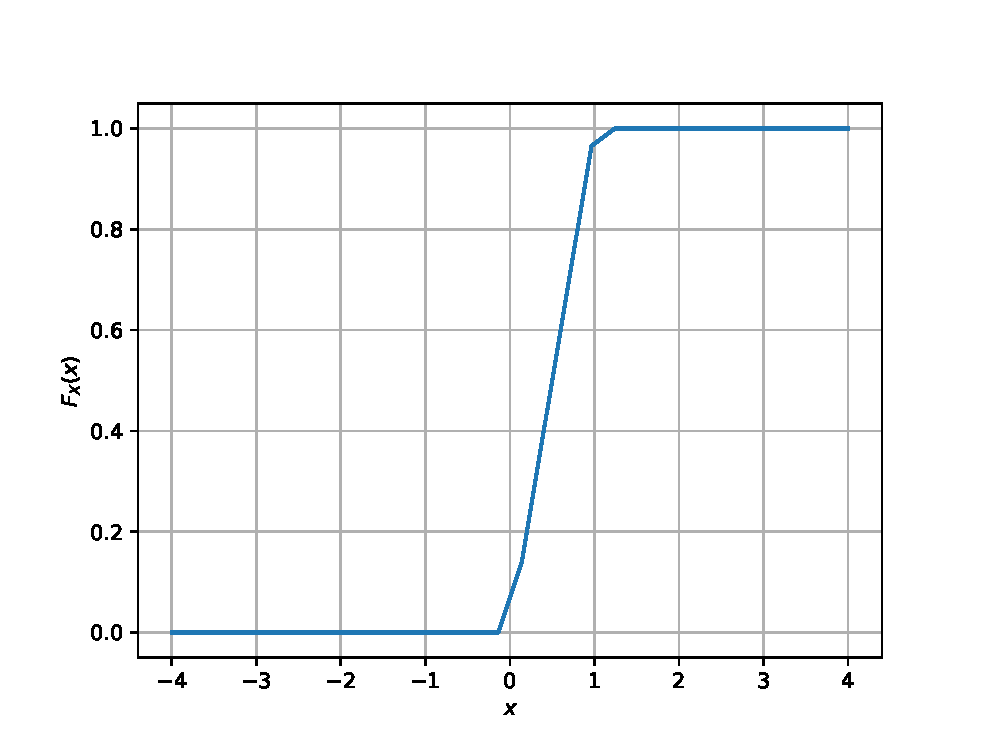
\includegraphics[width=\columnwidth]{./figs/uni_cdf}
\caption{The CDF of $U$}
\label{fig:uni_cdf}
\end{figure}

%
\item
Find a  theoretical expression for $F_{U}(x)$.\\
\textbf{Solution:} 
	Since it is uniform distribution then pdf is given by:
	\begin{equation}
		p_U(x)=
		\begin{cases}
        1 & 0 \le x\le 1 \\
	    0 & otherwise
		\end{cases}
	\end{equation}
	for $0<x<1 :$
	\begin{align}
		F_U(x) & = \int_{-\infty}^{x}p_U(x)dx  \\
		       & = \int_{0}^{x}1.dx \\
			   & = x
	\end{align}
	\begin{equation}
	F_U\brak{x}=\begin{cases}
	 0 & x<0 \\
	 x & 0\le x \le 1 \\
	 1 &1<x
\end{cases}	
	\end{equation}
	
\item
The mean of $U$ is defined as
%
\begin{equation}
E\sbrak{U} = \frac{1}{N}\sum_{i=1}^{N}U_i
\end{equation}
%
and its variance as
%
\begin{equation}
\text{var}\sbrak{U} = E\sbrak{U- E\sbrak{U}}^2 
\end{equation}

Write a C program to  find the mean and variance of $U$. \\
\textbf{Solution:}Download and excecute the code
\begin{lstlisting}
$ wget https://github.com/karna-rash/A11110-Assignment/blob/master/codes/1.3-1.4.c
\end{lstlisting}
Now compile and excecute
\begin{lstlisting}
$ gcc -o 1.3-1.4 1.3-1.4.c
$ ./1.3-1.4
\end{lstlisting}
Experimental values:
\begin{align}
\text{Mean} = 0.499772 \label{1.9}\\
\text{Variance}= 0.083368 \label{1.10}
\end{align}
\item Verify your result theoretically given that
\end{enumerate}
%
\begin{equation}
E\sbrak{U^k} = \int_{-\infty}^{\infty}x^kdF_{U}(x)
\end{equation}
\textbf{Solution:}
Mean and variance are given by :
\begin{align}
E\sbrak{U}&=\int_{0}^{1}x.dx=0.5\\
Var\sbrak{U}&=E\sbrak{U^2}-{E\sbrak{U}}^2=\int_{0}^{1}x^2.dx - 0 \\
&=\frac{1}{3} -\frac{1}{4} \\
&=\frac{1}{12}
\end{align}
By comparing these values obatined with results (\ref{1.9}) and (\ref{1.10}) we can conclude that simulation varies with theoritical analysis.
\section{Central Limit Theorem}
%
\begin{enumerate}[label=\thesection.\arabic*
,ref=\thesection.\theenumi]

%
\item
Generate $10^6$ samples of the random variable
%
\begin{equation}
X = \sum_{i=1}^{12}U_i -6
\end{equation}
%
using a C program, where $U_i, i = 1,2,\dots, 12$ are  a set of independent uniform random variables between 0 and 1
and save in a file called gau.dat\\
\textbf{Soltion:}Download 
\begin{lstlisting}
$ wget https://github.com/karna-rash/A11110-Assignment/blob/master/codes/2.1.c
$ wget https://github.com/karna-rash/A11110-Assignment/blob/master/codes/2.1.py
\end{lstlisting}
Now compile the c-code to generate the data
\begin{lstlisting}
$ gcc -o 2.1 2.1.c
$ ./2.1
\end{lstlisting}
Now excecute the python code which take the data from output of c  code:
\begin{lstlisting}
$ python3 2.1.py
\end{lstlisting}
%
\item
Load gau.dat in python and plot the empirical CDF of $X$ using the samples in gau.dat. What properties does a CDF have?
\\
\solution The CDF of $X$ is plotted in Fig. \ref{fig:gauss_cdf}
Properties:
\begin{enumerate}
\item it is symmetric about $\brak{0,0.5}$
\item its tends to one as we approch $x=6$
\end{enumerate}
\begin{lstlisting}
$ wget https://github.com/karna-rash/A11110-Assignment/blob/master/codes/2.2.py
$ python3 2.2.py
\end{lstlisting}
\begin{align}
Q\brak{x}&=\int_{x}^{\infty} exp\brak{\frac{-x^2}{2}}dx \\
erf\brak{x}&=\int_{0}^{x}exp\brak{\frac{-x^2}{2}}dx \\
F_X\brak{x}&=\int_{-\infty}^{x}exp\brak{\frac{-x^2}{2}}dx\\
F_X\brak{x}&=1-Q\brak{x}\\
Q\brak{x}&=\frac{1}{2}\brak{1-erf\brak{\frac{x}{\sqrt{2}}}}
\end{align}
\begin{figure}
\centering
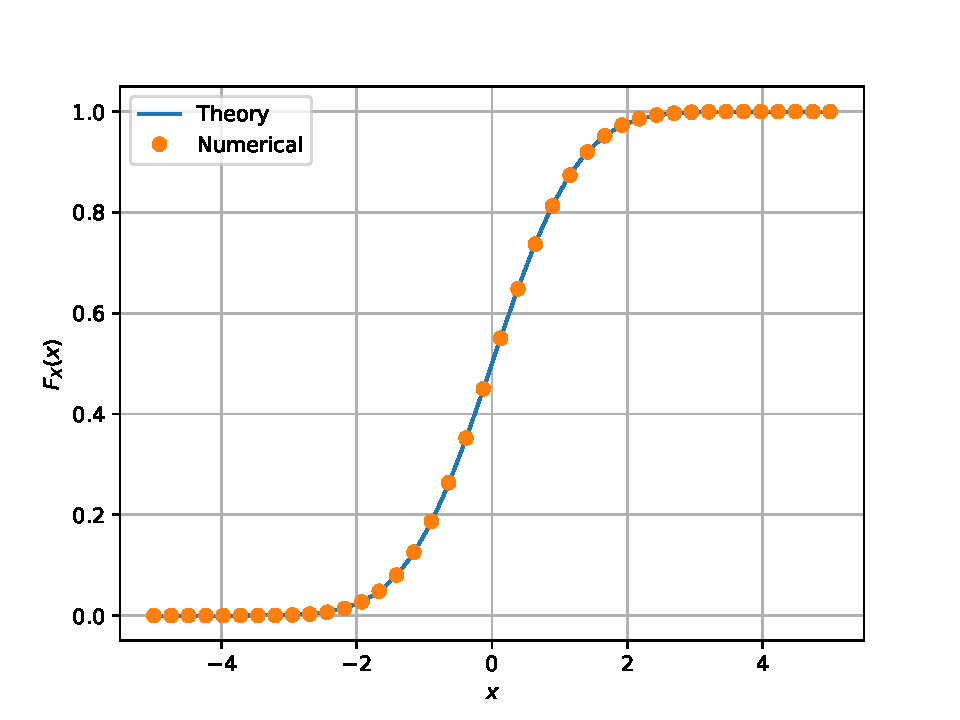
\includegraphics[width=\columnwidth]{./figs/gauss_cdf}
\caption{The CDF of $X$}
\label{fig:gauss_cdf}
\end{figure}
\item
Load gau.dat in python and plot the empirical PDF of $X$ using the samples in gau.dat. The PDF of $X$ is defined as
\begin{align}
p_{X}(x) = \frac{d}{dx}F_{X}(x)
\end{align}
What properties does the PDF have?
\\
\textbf{Solution:} The PDF of $X$ is plotted in Fig. \ref{fig:gauss_pdf} using the code below\\
Properties:
\begin{enumerate}
\item it is symmetric about $x=0$
\item its tends to zero as we approch $x=6$
\end{enumerate}
\begin{lstlisting}
$ wget https://github.com/karna-rash/A11110-Assignment/blob/master/codes/2.3.py
$ python3 2.3.py
\end{lstlisting}
\begin{figure}
\centering
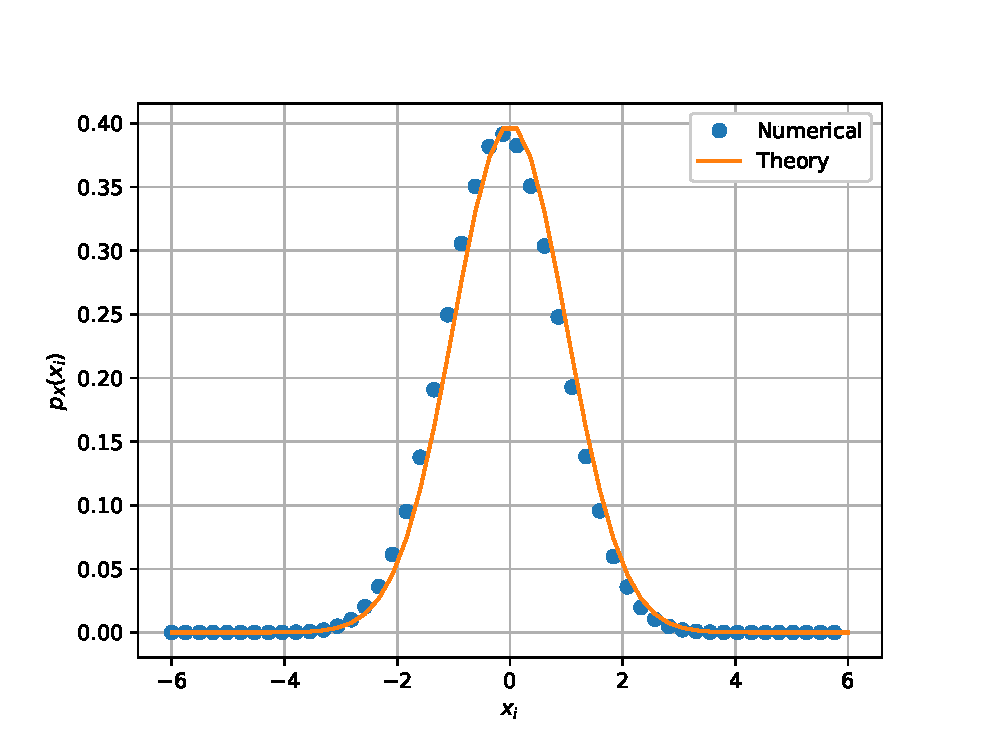
\includegraphics[width=\columnwidth]{./figs/gauss_pdf}
\caption{The PDF of $X$}
\label{fig:gauss_pdf}
\end{figure}

\item Find the mean and variance of $X$ by writing a C program.\\
\textbf{Solution:}
\begin{lstlisting}
wget https://github.com/karna-rash/A11110-Assignment/blob/master/codes/gau_mean.c
\end{lstlisting}
compile and execute:
\begin{lstlisting}
gcc -o gau_mean gau_mean.c -lm
./gau_mean
\end{lstlisting}
Experimental values
\begin{align}
\text{Mean} = -0.000354 \label{2.3}\\
\text{Variance}=1.001179 \label{2.4}
\end{align}
\item Given that 
\begin{align}
p_{X}(x) = \frac{1}{\sqrt{2\pi}}\exp\brak{-\frac{x^2}{2}}, -\infty < x < \infty,
\end{align}
repeat the above exercise theoretically.\\
\textbf{Solution:}
\begin{enumerate}
\item Mean :
\begin{align}
\e{X}&=\int_{-\infty}^{\infty}xp_X(x)dx \\
&=\int_{-\infty}^{\infty}\frac{1}{\sqrt{2\pi}}xexp\brak{-\frac{x^2}{2}}dx \\
&=-\frac{1}{\sqrt{2\pi}}\int_{-\infty}^{\infty}d\brak{exp\brak{-\frac{x^2}{2}}} \\
&=0
\end{align}
\item variance:
\begin{align}
\e{X^2}&=\int_{-\infty}^{\infty}x^2p_X(x)dx \\
&=\int_{-\infty}^{\infty}\frac{1}{\sqrt{2\pi}}x^2exp\brak{-\frac{x^2}{2}}dx \\
&=\frac{1}{\sqrt{2\pi}}\brak{x\int x exp\brak{-\frac{x^2}{2}}dx}
\\ &-\frac{1}{\sqrt{2\pi}}\int \int \brak{x exp\brak{-\frac{x^2}{2}}}dx. dx\\
&=\frac{1}{\sqrt{2\pi}}\int_{-\infty}^{\infty}exp\brak{-\frac{x^2}{2}}dx \\
&=\frac{\sqrt{2\pi}}{\sqrt{2\pi}}\\&=1
\end{align}
\end{enumerate}
By comparing these values obatined with results (\ref{2.3}) and (\ref{2.4}) we can conclude that simulation varies with theoritical analysis.
\end{enumerate}
\section{From Uniform to Other}
\begin{enumerate}[label=\thesection.\arabic*
,ref=\thesection.\theenumi]
%
\item
Generate samples of 
%
\begin{equation}
V = -2\ln\brak{1-U}
\end{equation}
%
and plot its CDF.\\
\textbf{Solution:}
Download the codes \ref{fig:vni_cdf}
\begin{lstlisting}
$ wget https://github.com/karna-rash/A11110-Assignment/blob/master/codes/3.1.c
$ wget https://github.com/karna-rash/A11110-Assignment/blob/master/codes/3.1.py
\end{lstlisting}
Compile and execute:
\begin{lstlisting}
$gcc -o 3.1 3.1.c
$./3.1
$python 3.1.py
\end{lstlisting}
\begin{figure}
\centering
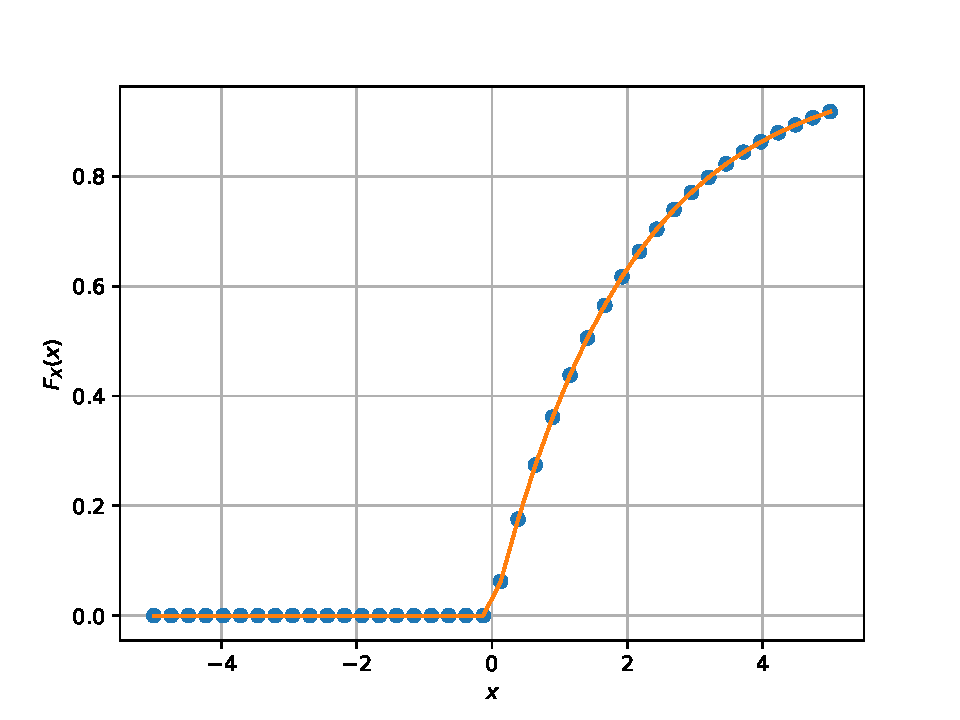
\includegraphics[width=\columnwidth]{./figs/vni_cdf}
\caption{The PDF of $V$}
\label{fig:vni_cdf}
\end{figure}
\item Find a theoretical expression for $F_V(x)$.
\textbf{Soltion:}
Let $V=G(U)$ then
\begin{align}
F_V(x)&=F_U(G^{-1}(x))\\
&=F_U(1-e^{-\frac{x}{2}}) \\
\end{align}
\begin{equation}
F_V(x)=
\begin{cases}
G^{-1}(x) & 0 \le 1-e^{-\frac{x}{2}} \le 1 \\
0 &  1-e^{-\frac{x}{2}} < 0
\end{cases}
\end{equation}
\begin{equation}
F_V(x)=
\begin{cases}
1-e^{-\frac{x}{2}} & 0 \le x \le \infty \\
0 &  x < 0
\end{cases}
\end{equation}
%
%\item
%Generate the Rayleigh distribution from Uniform. Verify your result through graphical plots.
\end{enumerate}
\section{Triangular Distribution}
\begin{enumerate}[label=\thesection.\arabic*
,ref=\thesection.\theenumi]
%
\item Generate 
	\begin{align}
		T = U_1+U_2
	\end{align}
	\textbf{Solution:}
	Download and excecute the code
	\begin{lstlisting}
$ wget https://github.com/karna-rash/A11110-Assignment/blob/master/codes/4.1.c
$ wget https://github.com/karna-rash/A11110-Assignment/blob/master/codes/functions.h
$ gcc 4.1.c -lm 
$ ./a.out 
	\end{lstlisting}
\item Find the CDF of $T$.\\
\textbf{Solution:}
Download and excecute the code .it gives the following plot Fig.\ref{fig:tri_cdf}
\begin{lstlisting}
$ wget https://github.com/karna-rash/A11110-Assignment/blob/master/codes/4.2.py
$ python 4.2.py
	\end{lstlisting}
	\begin{figure}
\centering
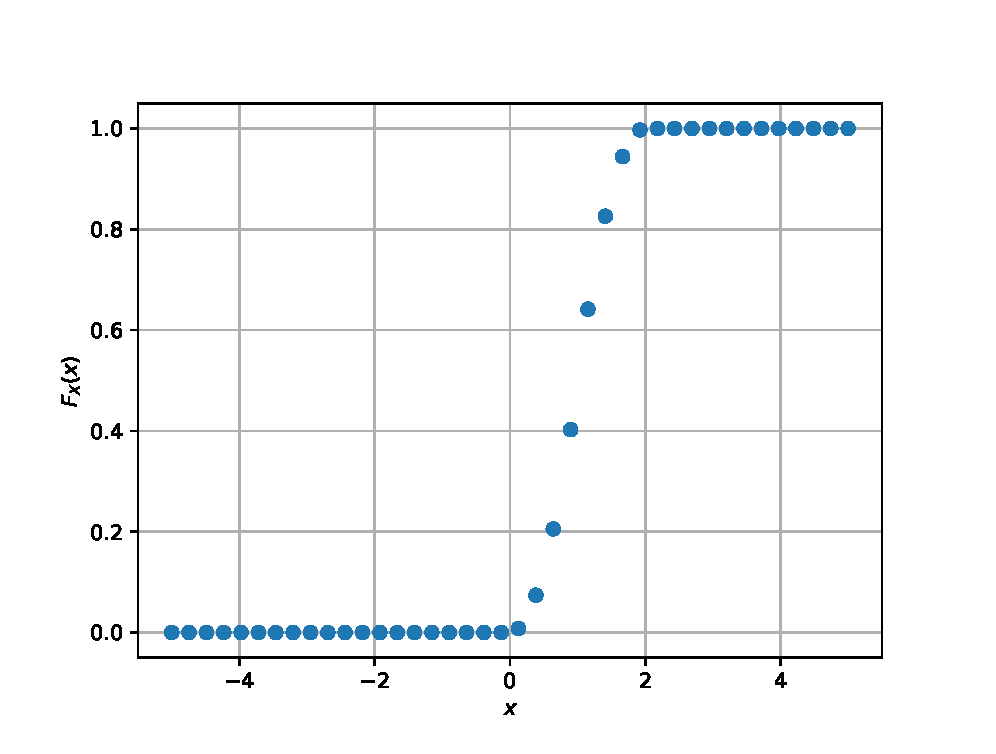
\includegraphics[width=\columnwidth]{./figs/tri_cdf}
\caption{The CDF of $T$}
\label{fig:tri_cdf}
\end{figure}
\item Find the PDF of $T$.\\
\textbf{Solution:}
Download and excecute the code. It gives the following plot Fig.\ref{fig:tri_pdf}
\begin{lstlisting}
$ wget https://github.com/karna-rash/A11110-Assignment/blob/master/codes/4.3.py
$ python 4.3.py
\end{lstlisting}
\begin{figure}
\centering
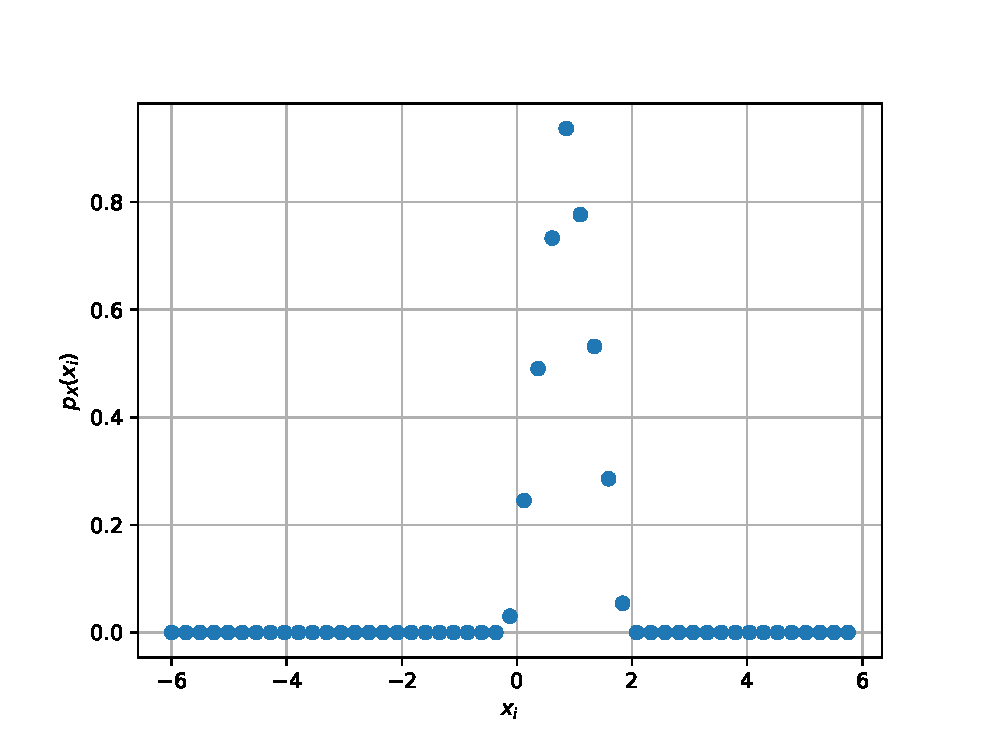
\includegraphics[width=\columnwidth]{./figs/tri_pdf}
\caption{The PDF of $T$}
\label{fig:tri_pdf}
\end{figure}
\textbf{Solution:}
Download and excecute the code. It gives the following plot Fig.\ref{fig:tri_cdf}
\item Find the theoretical expressions for the PDF and CDF of $T$.\\
\textbf{Solution:}
Let us use convulsion of $p_{U_1}\brak{x} \text{and} p_{U_2}\brak{x}$
\begin{align}
p_T\brak{t}=\int_{-\infty}^{\infty}p_{U_1}\brak
{T-\alpha}p_{U_2}\brak{\alpha} d \alpha
\end{align}
\begin{equation}
p_T\brak{t}=
\begin{cases}
\int_{0}^{t} 1.d\alpha & 0 \le t <1 \\
\int_{t-1}^{1}1.d\alpha & 1\le t \le2 \\
0 & otherwise
\end{cases}
\end{equation}
\begin{equation}
 =\begin{cases}
t & 0 \le t <1 \\
2-t & 1\le t \le2 \\
0 & otherwise
\end{cases}
\end{equation}
Now we can get CDF from PDF
\begin{align}
F_T\brak{t}&=\pr{T\le t} \\
&=\int_{-\infty}^{t}p_T\brak{x}dx
\end{align}
\begin{equation}
F_T\brak{t} =\begin{cases}
0 & t \le 0 \\
\int_{0}^{t}x.dx & 0 \le t <1 \\
\int_{1}^{t}2-x.dx + \frac{1}{2}& 1\le t \le2 \\
1 & 2 \le t
\end{cases}
\end{equation}
\begin{equation}
=\begin{cases}
0 & t \le 0 \\
\frac{x^2}{2} & 0 \le t <1 \\
\frac{\brak{2-x}^2}{2} & 1\le t \le2 \\
1 & 2 \le t
\end{cases}
\end{equation}
\item Verify your results through a plot. \\
\textbf{Solution:}
After Compare the empirical and theorical plots in \ref{fig:tri_cdf_verify} and \ref{fig:tri_pdf_verify}
\begin{figure}
\centering
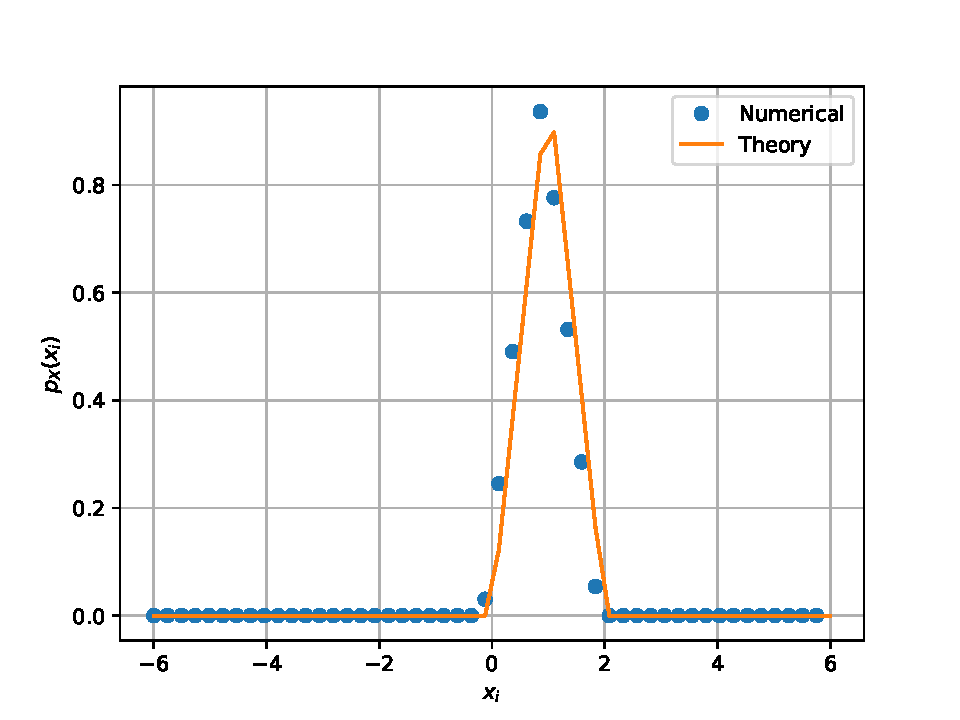
\includegraphics[width=\columnwidth]{./figs/tri_pdf_verify}
\caption{The PDF verify of $T$}
\label{fig:tri_pdf_verify}
\end{figure}
\begin{figure}
\centering
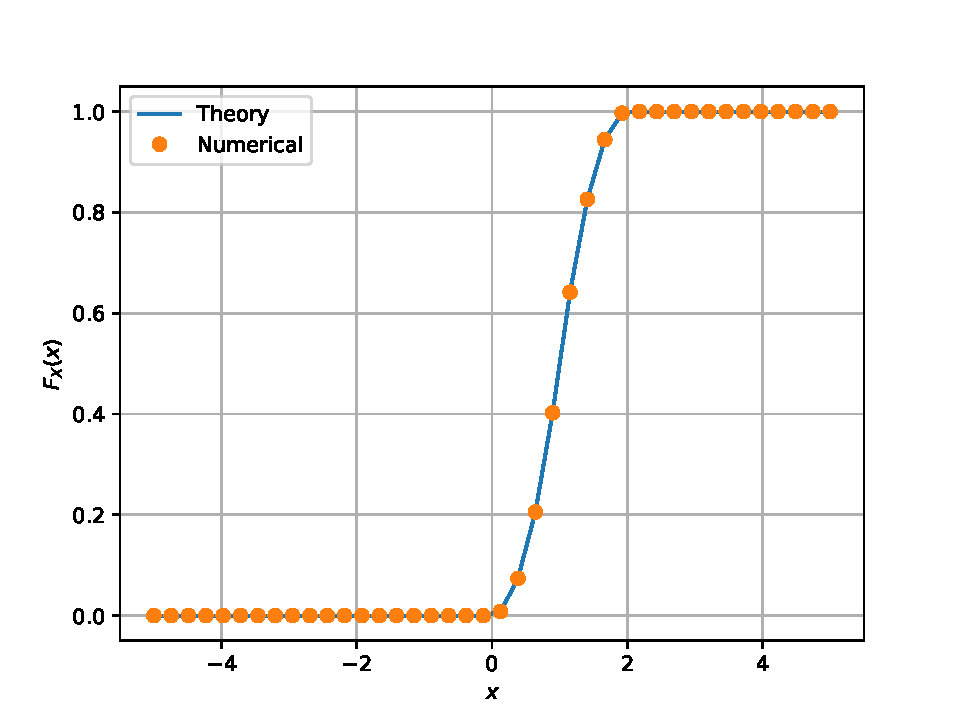
\includegraphics[width=\columnwidth]{./figs/tri_cdf_verify}
\caption{The CDF Verify of $T$}
\label{fig:tri_cdf_verify}
\end{figure}
\end{enumerate}
\section{Maximum Likelihood}
\begin{enumerate}[label=\thesection.\arabic*
,ref=\thesection.\theenumi]
\item Generate equiprobable $X \in \cbrak{1,-1}$.
\textbf{Solution:}
	Download and excecute the code
	\begin{lstlisting}
$ wget https://github.com/karna-rash/A11110-Assignment/blob/master/codes/5.1.c
$ wget https://github.com/karna-rash/A11110-Assignment/blob/master/codes/functions.h
$ gcc 5.1.c -lm 
$ ./a.out 
	\end{lstlisting}
\item Generate 
\begin{equation}
Y = AX+N,
\end{equation}
		where $A = 5$ dB,  and $N \sim \mathcal{N}\brak{0,1}$.
		\textbf{Solution:}
	Download and excecute the code
	\begin{lstlisting}
$ wget https://github.com/karna-rash/A11110-Assignment/blob/master/codes/5.2.c
$ wget https://github.com/karna-rash/A11110-Assignment/blob/master/codes/functions.h
$ gcc 5.2.c -lm 
$ ./a.out 
	\end{lstlisting}
	\item Plot $Y$ using a scatter plot.
	\item Guess how to estimate $X$ from $Y$.
\item
\label{ml-ch4_sim}
Find 
\begin{equation}
	P_{e|0} = \pr{\hat{X} = -1|X=1}
\end{equation}
and 
\begin{equation}
	P_{e|1} = \pr{\hat{X} = 1|X=-1}
\end{equation}
%
\item Find $P_e$ assuming that $X$ has equiprobable symbols.
%
\item
Verify by plotting  the theoretical $P_e$ with respect to $A$ from 0 to 10 dB.  
%
\item Now, consider a threshold $\delta$  while estimating $X$ from $Y$. Find the value of $\delta$ that maximizes the theoretical $P_e$.
\item Repeat the above exercise when 
	\begin{align}
		p_{X}(0) = p
	\end{align}
\item Repeat the above exercise using the MAP criterion.
		\end{enumerate}
\end{document}

